% =====================================================================
%  Project A report - AIAA conference paper layout
%  Author: Maxat Bekmurzayev
%
%  Compile:  pdflatex report.tex   (run twice)
%  Figures are read from ../../Figures
% =====================================================================
\documentclass[letterpaper,10pt]{article}

\usepackage[margin=1in]{geometry}
\usepackage[T1]{fontenc}
\usepackage{mathptmx}
\usepackage{amsmath}
\usepackage{bm}
\usepackage{graphicx}
\usepackage{booktabs}
\usepackage{array}
\usepackage{float}
\usepackage[labelsep=space,labelfont=bf,font=small]{caption}
\usepackage{subcaption}
\usepackage{titlesec}
\usepackage{enumitem}
\usepackage{xcolor}
\usepackage[hidelinks]{hyperref}

\graphicspath{{../../Figures/}}

\renewcommand{\thesection}{\Roman{section}}
\renewcommand{\thesubsection}{\Alph{subsection}}
\renewcommand{\thesubsubsection}{\arabic{subsubsection}}
\titleformat{\section}[block]{\centering\normalsize\bfseries}{\thesection.}{0.5em}{}
\titleformat{\subsection}[block]{\normalsize\bfseries}{\thesubsection.}{0.5em}{}
\titleformat{\subsubsection}[block]{\normalsize\itshape}{\thesubsubsection.}{0.5em}{}
\titlespacing*{\section}{0pt}{12pt}{6pt}
\titlespacing*{\subsection}{0pt}{9pt}{4pt}

\captionsetup[figure]{name=Fig.}
\setlength{\parskip}{0pt}
\setlength{\parindent}{1.5em}

\newcommand{\figref}[1]{Fig.~\ref{#1}}
\newcommand{\vv}[1]{\bm{#1}}
\newcommand{\Tp}{^{\mathsf{T}}}

% =====================================================================
\begin{document}

\begin{center}
{\LARGE\bfseries Quaternion-Based Attitude Dynamics and Control\\[2pt]
of a 3U CubeSat\par}
\vspace{12pt}
{\large Maxat Bekmurzayev\footnote{Undergraduate student, L.~N.~Gumilyov Eurasian National University, Astana, Kazakhstan.}\par}
\end{center}

\vspace{6pt}
\begin{quote}
\bfseries
This report describes a MATLAB simulation of attitude control for a 3U
CubeSat with three reaction wheels. The attitude is described with
quaternions, the rotational motion with Euler's equations, and the controller
is a PD law on the quaternion error with a torque limit of 1~mN$\cdot$m per
axis. The test case is a satellite that starts with a tumble of
$19.7^\circ$/s and has to turn by $120^\circ$ to a fixed target attitude. The
controller reaches the target within $0.11^\circ$ and $0.01^\circ$/s in
74.1~s, and the wheels saturate only during the first 5.6~s. The results were
checked in three ways: the quaternion norm stays at $1$ to machine precision,
a fixed-step RK4 solution and an \texttt{ode45} solution differ by at most
$1.3\times10^{-4}$ degrees, and a Lyapunov function decreases monotonically.
The Lyapunov check also helped me find an error in the first version of the
code. Finally, the attitude was estimated from noisy sun sensor and
magnetometer vectors with the TRIAD method, with an RMS error of $0.60^\circ$.
\end{quote}

% ---------------------------------------------------------------------
\section*{Nomenclature}
\begin{tabular}{@{}l@{\hspace{1.2em}=\hspace{1.2em}}l@{}}
$\vv{q} = [\vv{\varepsilon}\Tp,\ \eta]\Tp$ & attitude quaternion (vector part, scalar part) \\
$\vv{q}_d$, $\vv{q}_e$ & target quaternion, error quaternion \\
$\vv{\omega}$ & angular velocity in body frame, rad/s \\
$\vv{\tau}$ & control torque, N$\cdot$m \\
$\vv{J}$ & inertia matrix, kg$\cdot$m$^2$ \\
$K_p$, $K_d$ & proportional and derivative gains \\
$V$ & Lyapunov function \\
$\omega_n$, $\zeta$ & natural frequency, damping ratio \\
$[\vv{a}\times]$ & skew-symmetric matrix, $[\vv{a}\times]\vv{b} = \vv{a}\times\vv{b}$ \\
\end{tabular}

% =====================================================================
\section{Introduction}

Almost every spacecraft has to control its orientation. Cameras must look at
the ground target, antennas must point at the ground station, and solar
panels must face the Sun. The subsystem that does this is the attitude
determination and control system (ADCS) \cite{wertz,wie}. For CubeSats the
problem is harder than for large satellites, because the actuators are small
and the power is limited.

The orientation can be described with Euler angles, but the 3-2-1 sequence
has a singularity at a pitch angle of $\pm90^\circ$ (gimbal lock), where the
kinematic equations contain $\sec\theta$ \cite{shuster}. A satellite that
must make large turns can reach this region. Quaternions use four parameters
instead of three and have no such singularity, so they are the usual choice
in ADCS software \cite{markley,wie_barba}.

The goals of this project were:
\begin{enumerate}[leftmargin=2.2em,itemsep=0pt]
  \item write the quaternion kinematics and Euler's equations for a 3U CubeSat;
  \item design a PD controller on the quaternion error and check its stability;
  \item simulate a detumble plus a $120^\circ$ turn in MATLAB with my own RK4
        integrator and check the results;
  \item estimate the attitude from two noisy vector measurements (TRIAD).
\end{enumerate}

% =====================================================================
\section{Mathematical Model}

\subsection{Frames and Quaternions}

Two frames are used: the Earth-centered inertial frame (ECI) and the body
frame, which is fixed to the satellite with its origin at the center of mass
and its axes along the principal axes of inertia. The $z_B$ axis is along the
long (30~cm) side of the CubeSat.

A rotation by angle $\phi$ about a unit axis $\hat{\vv{e}}$ is written as the
quaternion
\begin{equation}
  \vv{\varepsilon} = \hat{\vv{e}}\sin\frac{\phi}{2}, \qquad \eta = \cos\frac{\phi}{2},
  \qquad \vv{\varepsilon}\Tp\vv{\varepsilon} + \eta^2 = 1 .
  \label{eq:quat}
\end{equation}
The matching direction cosine matrix, used only for plots and sensor
modeling, is
\begin{equation}
  \vv{C}(\vv{q}) = (\eta^2 - \vv{\varepsilon}\Tp\vv{\varepsilon})\vv{I}_3
  + 2\vv{\varepsilon}\vv{\varepsilon}\Tp - 2\eta[\vv{\varepsilon}\times].
\end{equation}

\subsection{Kinematics}

If $\vv{\omega}$ is the body angular velocity, the quaternion changes as
\cite{markley}
\begin{equation}
  \dot{\vv{q}} = \frac{1}{2}\,\Xi(\vv{q})\,\vv{\omega}, \qquad
  \Xi(\vv{q}) = \begin{bmatrix} \eta\vv{I}_3 + [\vv{\varepsilon}\times] \\ -\vv{\varepsilon}\Tp \end{bmatrix}.
  \label{eq:kin}
\end{equation}
It is easy to show that $\vv{q}\Tp\Xi(\vv{q}) = \vv{0}\Tp$, so
$d(\vv{q}\Tp\vv{q})/dt = 0$: the exact equation keeps the norm equal to one.
A numerical integrator does not keep it exactly, so in the code the
quaternion is normalized after every step.

\subsection{Dynamics}

For a rigid body with angular momentum $\vv{H} = \vv{J}\vv{\omega}$, the
derivative in the rotating body frame gives Euler's equation \cite{hughes}
\begin{equation}
  \vv{J}\dot{\vv{\omega}} = \vv{\tau} - \vv{\omega}\times(\vv{J}\vv{\omega}).
  \label{eq:euler}
\end{equation}
The last term is the gyroscopic coupling. It is zero only when $\vv{\omega}$
is along a principal axis or when all three moments of inertia are equal. For
the CubeSat $J_x = J_y \ne J_z$, so the transverse rates exchange momentum
during a maneuver. Disturbance torques (gravity gradient, drag, magnetic,
solar pressure) are not included, so $\vv{\tau}$ is only the control torque.

Equations~(\ref{eq:kin}) and (\ref{eq:euler}) together give a 7-state model
$\vv{x} = [\vv{q}\Tp,\ \vv{\omega}\Tp]\Tp$.

% =====================================================================
\section{Spacecraft Parameters}

The satellite is a 3U CubeSat of $10\times10\times30$~cm with the maximum
mass of 4.0~kg allowed by the CubeSat specification \cite{cds}. I assumed a
uniform mass distribution and the center of mass at the geometric center.
For a uniform box,
\begin{equation}
  J_x = J_y = \frac{m}{12}(b^2 + c^2) = 0.0333~\mathrm{kg\,m^2}, \qquad
  J_z = \frac{m}{12}(a^2 + b^2) = 0.00667~\mathrm{kg\,m^2}.
\end{equation}
A real CubeSat has batteries, boards and wheels in different places, so the
real values would be somewhat different and there would be small products of
inertia. The main parameters are listed in Table~\ref{tab:params}.

\begin{table}[htbp]
\centering
\caption{Spacecraft and simulation parameters.}
\label{tab:params}
\begin{tabular}{@{}lc@{}}
\toprule
Parameter & Value \\
\midrule
Mass & 4.0 kg \\
Inertia & diag(0.0333, 0.0333, 0.00667) kg$\cdot$m$^2$ \\
Wheel torque limit (per axis) & 1.0 mN$\cdot$m \\
Initial quaternion & $[0,\,0,\,0,\,1]\Tp$ \\
Initial angular velocity & $[10,\,-15,\,8]\Tp$ deg/s ($|\vv{\omega}| = 19.7$ deg/s) \\
Target quaternion & $[0.5,\,0.5,\,0.5,\,0.5]\Tp$ ($120^\circ$ about $[1,1,1]/\sqrt3$) \\
Simulation time, step & 120 s, 0.01 s \\
\bottomrule
\end{tabular}
\end{table}

The main assumptions are: rigid body, no disturbance torques, each wheel is
an ideal torque source with a saturation limit (wheel momentum is not
tracked), and the controller knows the exact attitude and rate.

% =====================================================================
\section{Controller Design}

\subsection{Error Quaternion}

The target is a fixed attitude $\vv{q}_d$ with zero rate. The attitude error
is written as a quaternion
\begin{equation}
  \vv{q}_e = \vv{q}_d^{-1}\otimes\vv{q}, \qquad
  \vv{\varepsilon}_e = \eta_d\vv{\varepsilon} - \eta\vv{\varepsilon}_d - [\vv{\varepsilon}_d\times]\vv{\varepsilon}, \qquad
  \eta_e = \eta\eta_d + \vv{\varepsilon}\Tp\vv{\varepsilon}_d .
  \label{eq:qerr}
\end{equation}
At the target $\vv{\varepsilon}_e = \vv{0}$ and $\eta_e = 1$. With this order
of multiplication and a constant $\vv{q}_d$, the error quaternion follows the
same kinematics as $\vv{q}$, $\dot{\vv{q}}_e = \frac12\Xi(\vv{q}_e)\vv{\omega}$.
This is needed for the stability proof below.

\subsection{PD Control Law}

The control torque is
\begin{equation}
  \vv{\tau} = -K_p\,\mathrm{sgn}(\eta_e)\,\vv{\varepsilon}_e - K_d\,\vv{\omega},
  \label{eq:pd}
\end{equation}
and each component is limited to $\pm1$~mN$\cdot$m. The factor
$\mathrm{sgn}(\eta_e)$ is needed because $\vv{q}_e$ and $-\vv{q}_e$ describe
the same attitude. Without it the satellite can turn the long way, almost a
full revolution, which is called unwinding \cite{bhat}.

\subsection{Stability}

As a Lyapunov function I used \cite{wie_barba}
\begin{equation}
  V = 2K_p(1 - |\eta_e|) + \frac12\vv{\omega}\Tp\vv{J}\vv{\omega}.
  \label{eq:V}
\end{equation}
$V$ is zero only at the target with zero rate and positive everywhere else.
Using $\dot\eta_e = -\frac12\vv{\varepsilon}_e\Tp\vv{\omega}$ and
Eq.~(\ref{eq:euler}),
\begin{equation}
  \dot V = K_p\,\mathrm{sgn}(\eta_e)\,\vv{\varepsilon}_e\Tp\vv{\omega}
  + \vv{\omega}\Tp\vv{\tau} - \vv{\omega}\Tp\bigl(\vv{\omega}\times\vv{J}\vv{\omega}\bigr)
  = -K_d\,\vv{\omega}\Tp\vv{\omega} \le 0 .
  \label{eq:Vdot}
\end{equation}
The gyroscopic term is zero because $\vv{\omega}\Tp(\vv{\omega}\times\vv{a}) = 0$
for any vector $\vv{a}$, and the two $K_p$ terms cancel after substituting
Eq.~(\ref{eq:pd}). By LaSalle's principle the state goes to
$\vv{\varepsilon}_e = \vv{0}$, $\vv{\omega} = \vv{0}$ for any positive gains.
This holds without saturation; with saturation the simulation result is used
as the check.

\subsection{Gain Selection}

For a small error, $\dot{\vv{\varepsilon}}_e \approx \frac12\vv{\omega}$ and
$J\dot\omega \approx \tau$, so each axis behaves like
\begin{equation}
  \ddot\varepsilon_e + \frac{K_d}{J}\dot\varepsilon_e + \frac{K_p}{2J}\varepsilon_e = 0
  \quad\Rightarrow\quad
  K_p = 2J\omega_n^2, \qquad K_d = 2\zeta\omega_n J .
  \label{eq:gains}
\end{equation}
I chose $\zeta = 0.7$ and a settling time of about 60~s, which gives
$\omega_n \approx 0.095$~rad/s. With the larger inertia $J = 0.0333$~kg$\cdot$m$^2$
this gives $K_p = 6.0\times10^{-4}$~N$\cdot$m and $K_d = 4.4\times10^{-3}$~N$\cdot$m$\cdot$s.
The same scalar gains are used on all three axes. Because $J_z$ is five times
smaller, the $z$ axis is more damped than $x$ and $y$. A per-axis version of
the gains is compared in Section~VI.

% =====================================================================
\section{Simulation}

The code is split into small MATLAB functions, one for each part of the
model (Table~\ref{tab:files}).

The state is integrated with the classical fourth-order Runge--Kutta method
with a fixed step of 0.01~s. The controller is evaluated inside every RK4
stage, so the closed loop is integrated, not a fixed torque history. After
each step the quaternion is divided by its norm. The step is much smaller
than the controller time scale ($1/\omega_n \approx 10.5$~s) and the initial
tumble time scale ($\approx 2.9$~s). As an independent check the same model
was also solved with MATLAB's \texttt{ode45}.

\begin{table}[htbp]
\centering
\caption{MATLAB files.}
\label{tab:files}
\begin{tabular}{@{}ll@{}}
\toprule
File & Purpose \\
\midrule
\texttt{cubesat\_params.m} & mass, inertia, torque limit, gains, initial conditions \\
\texttt{attitude\_dynamics.m} & state derivative, Eqs.~(\ref{eq:kin}) and (\ref{eq:euler}) \\
\texttt{pd\_controller.m} & error quaternion, PD law and saturation, Eqs.~(\ref{eq:qerr})--(\ref{eq:pd}) \\
\texttt{rk4\_integrator.m} & fixed-step RK4 with quaternion normalization \\
\texttt{quat\_to\_dcm.m}, \texttt{quat\_to\_euler321.m} & conversions for plots and sensors \\
\texttt{main\_simulation.m} & runs the simulation, \texttt{ode45} check and figures \\
\texttt{compare\_gain\_designs.m} & scalar vs per-axis gains \\
\texttt{sensor\_model.m}, \texttt{triad.m} & noisy sensors and TRIAD method \\
\texttt{determination\_demo.m} & attitude determination test \\
\bottomrule
\end{tabular}
\end{table}

% =====================================================================
\section{Results}

The main results are given in Table~\ref{tab:results}.

\begin{table}[htbp]
\centering
\caption{Main simulation results.}
\label{tab:results}
\begin{tabular}{@{}lc@{}}
\toprule
Quantity & Value \\
\midrule
Settling time ($|\vv{\varepsilon}_e| < 0.02$ and $|\vv{\omega}| < 0.01$ rad/s) & 74.1 s \\
Final attitude error $|\vv{\varepsilon}_e|$ & $9.6\times10^{-4}$ ($0.11^\circ$) \\
Final angular rate & 0.010 deg/s \\
Peak torque & 1.0 mN$\cdot$m (limit) \\
Time with saturation & first 5.6 s (4.7\% of the run) \\
Maximum quaternion norm error & $2.2\times10^{-16}$ \\
Maximum RK4 vs \texttt{ode45} difference & $1.3\times10^{-4}$ deg \\
\bottomrule
\end{tabular}
\end{table}

\subsection{Attitude and Angular Velocity}

\figref{fig:quat} shows the quaternion components. All four reach the target
value 0.5, but not monotonically: $q_2$ first goes down to about $-0.58$
before it turns and rises to 0.5. This is expected, because the maneuver
starts with both a large rate and a large attitude error, which is far from
the small-angle model used to choose the gains.

\begin{figure}[htbp]
\centering
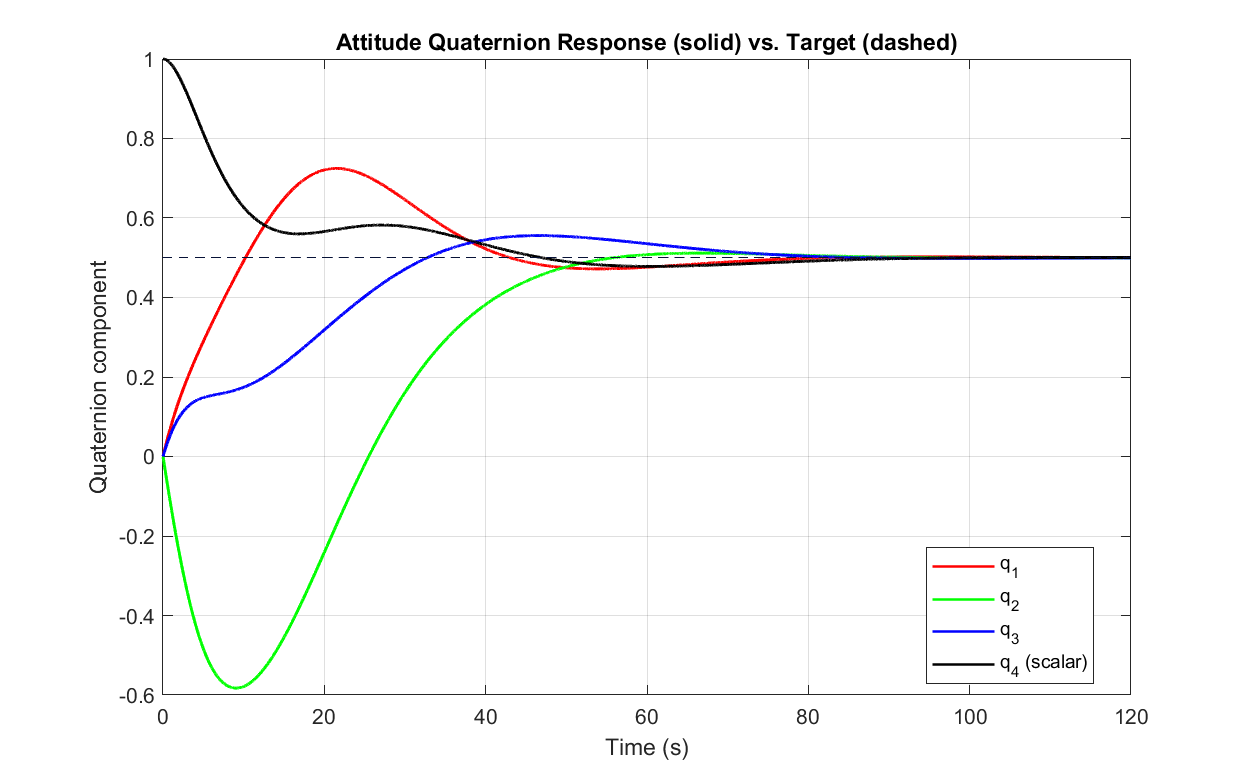
\includegraphics[width=0.82\textwidth]{fig_quaternion_response.png}
\caption{Quaternion components (solid) and target values (dashed).}
\label{fig:quat}
\end{figure}

The same motion in 3-2-1 Euler angles is shown in \figref{fig:euler}. The
roll angle overshoots to about $118^\circ$ and the pitch angle swings to about
$-68^\circ$ before the final attitude $(90^\circ, 0^\circ, 90^\circ)$ is
reached. In this run the pitch does not reach $\pm90^\circ$, but the Euler
angles change much more than the quaternion components, which always stay
between $-1$ and $1$. The Euler angles are only computed for plotting.

\begin{figure}[htbp]
\centering
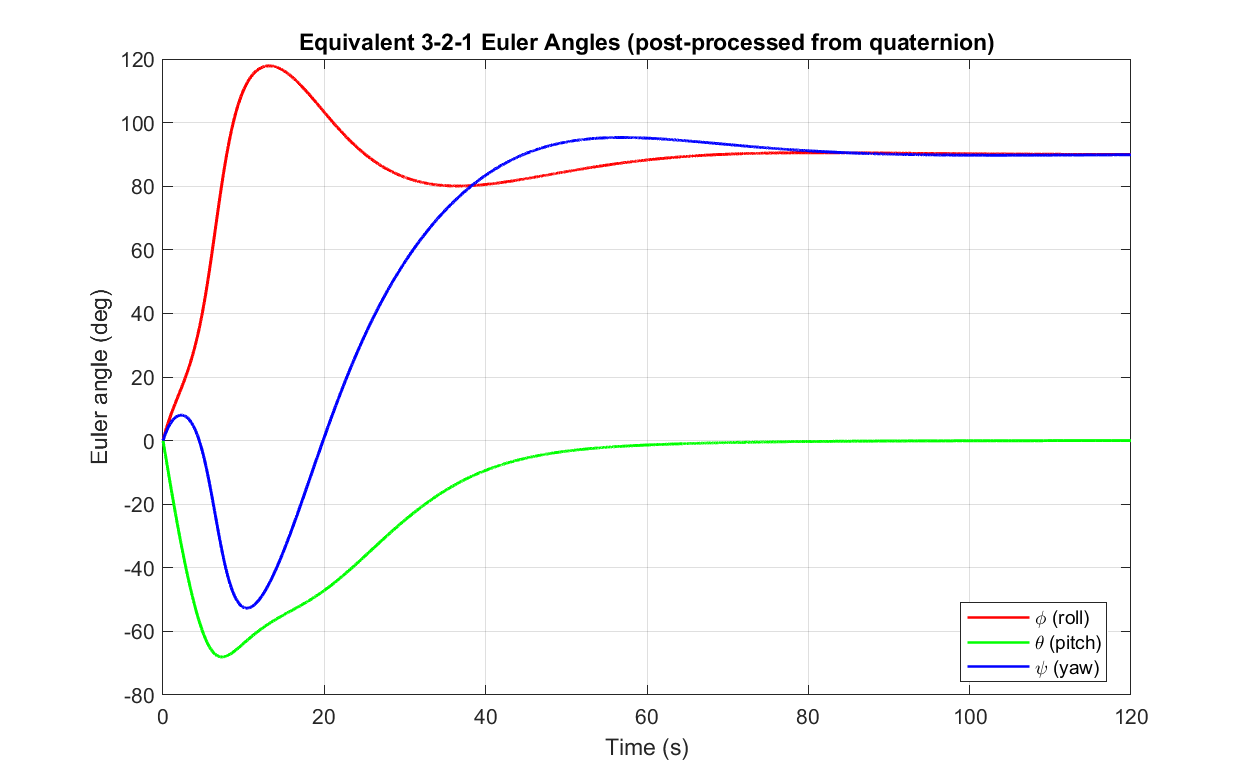
\includegraphics[width=0.82\textwidth]{fig_euler_angles.png}
\caption{Equivalent 3-2-1 Euler angles (computed only for plotting).}
\label{fig:euler}
\end{figure}

\begin{figure}[htbp]
\centering
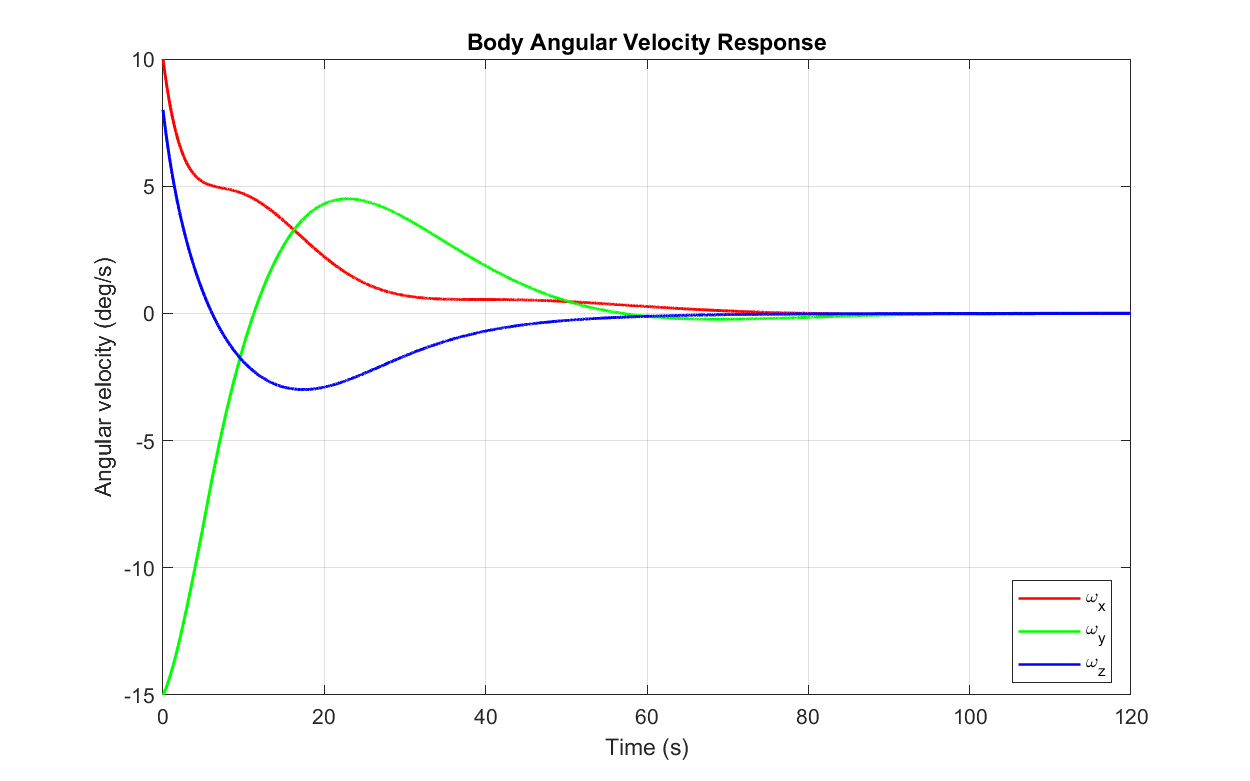
\includegraphics[width=0.82\textwidth]{fig_angular_velocity.png}
\caption{Body angular velocity.}
\label{fig:rate}
\end{figure}

The angular velocity (\figref{fig:rate}) also does not decay as one simple
exponential. $\omega_x$ slows its decay between about 5 and 15~s, and
$\omega_y$ changes sign and reaches a second peak of about 4.5~deg/s near
23~s. This is the effect of the gyroscopic term in Eq.~(\ref{eq:euler}),
which moves angular momentum between the transverse axes.

\subsection{Control Torque}

The wheel torques are shown in \figref{fig:torque}. The $y$ wheel, which has
to stop the largest initial rate ($-15$~deg/s), stays at the 1~mN$\cdot$m
limit for the first 5.6~s. After that all torques are below the limit and
go smoothly to zero. I did not tune the gains to avoid saturation, so that
the saturation part of the code is also tested.

\begin{figure}[htbp]
\centering
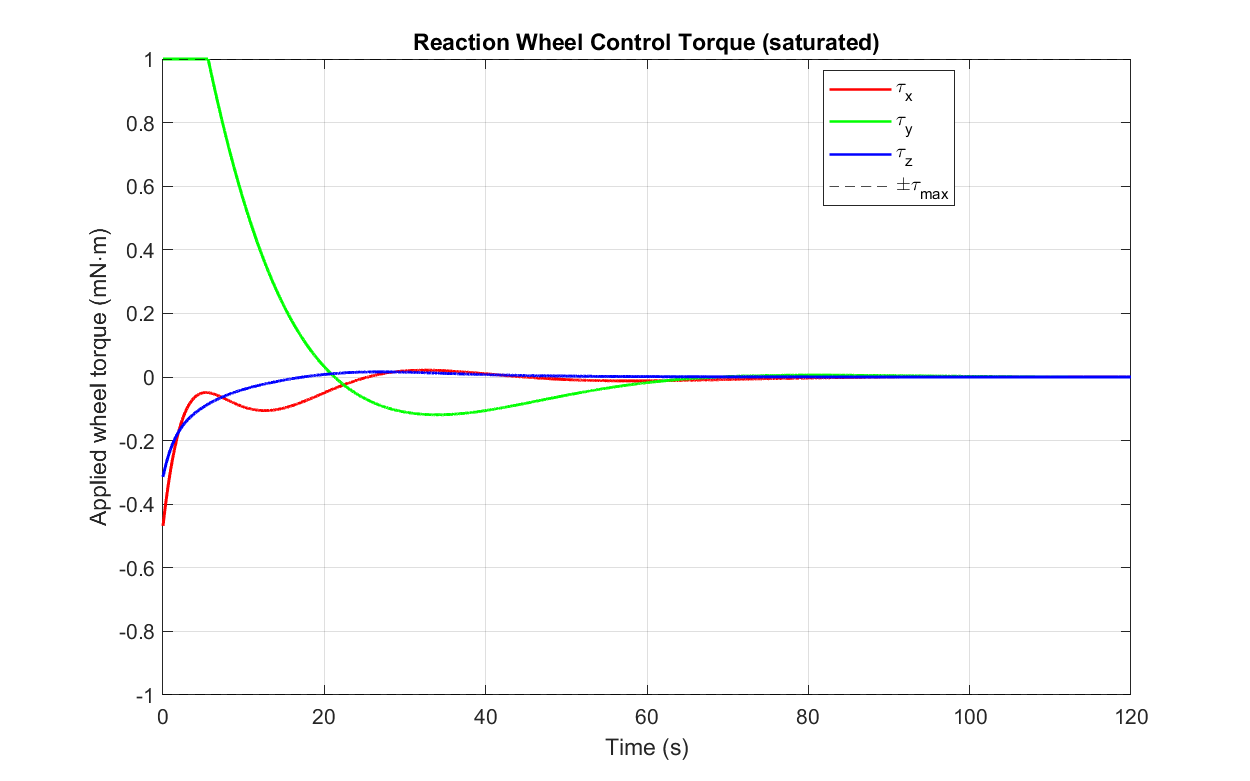
\includegraphics[width=0.82\textwidth]{fig_control_torque.png}
\caption{Wheel torque per axis. Dashed lines show the $\pm1$ mN$\cdot$m limit.}
\label{fig:torque}
\end{figure}

The settling time of 74.1~s is about 23\% longer than the 60~s used for the
gain design. This makes sense: the linear model does not include the large
initial error, the gyroscopic coupling or the saturation, and all three make
the response slower, not faster.

\subsection{Per-Axis Gains}

I also tried per-axis gains from Eq.~(\ref{eq:gains}) with each $J_i$, which
gives
\begin{equation*}
  K_p = \mathrm{diag}(6.0,\ 6.0,\ 1.2)\times10^{-4}~\mathrm{N\,m}, \qquad
  K_d = \mathrm{diag}(4.4,\ 4.4,\ 0.88)\times10^{-3}~\mathrm{N\,m\,s}.
\end{equation*}
With these gains all axes
have the same damping, but the settling time grows to 78.8~s and the final
error is $1.5\times10^{-3}$. The $z$ axis was overdamped with the scalar
gains, but it also had a higher bandwidth, so it was not slower. I kept the
scalar gains as the baseline.

% =====================================================================
\section{Validation}

\subsection{Lyapunov Function}

\figref{fig:lyap} shows $V(t)$ from Eq.~(\ref{eq:V}) along the simulated
trajectory. It decreases monotonically by about six orders of magnitude, as
Eq.~(\ref{eq:Vdot}) predicts. The slope becomes smaller between about 45 and
65~s, where $|\vv{\omega}|$ is small, because $\dot V = -K_d|\vv{\omega}|^2$.

\begin{figure}[htbp]
\centering
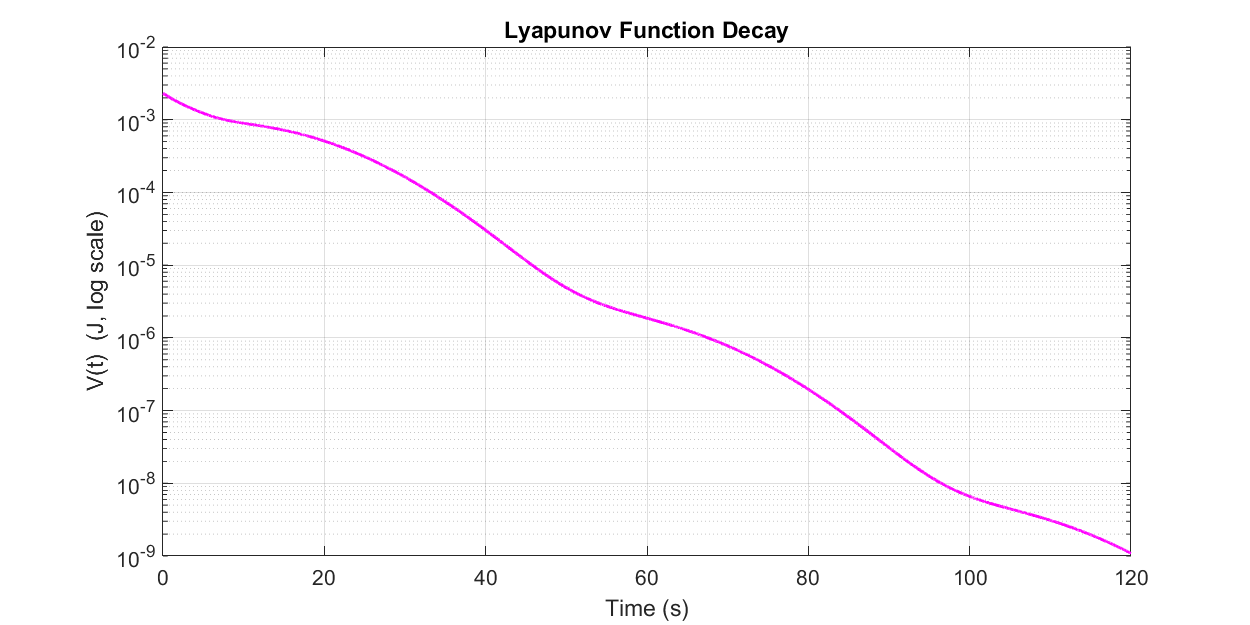
\includegraphics[width=0.72\textwidth]{fig_lyapunov.png}
\caption{Lyapunov function $V(t)$ on a log scale.}
\label{fig:lyap}
\end{figure}

This check was useful in practice. In my first version of the code the error
quaternion was computed as $\vv{q}\otimes\vv{q}_d^{-1}$ instead of
$\vv{q}_d^{-1}\otimes\vv{q}$. This is also a valid attitude error, and the
satellite still converged, but $V(t)$ went up and down several times during
the run. Since Eq.~(\ref{eq:Vdot}) says $V$ can never increase, the code had
to be wrong. The wrong order does not satisfy
$\dot{\vv{q}}_e = \frac12\Xi(\vv{q}_e)\vv{\omega}$ with the same
$\vv{\omega}$, and after fixing it $V(t)$ became monotonic.

\subsection{Quaternion Norm and Integrator Check}

\figref{fig:norm} shows that $\bigl|\,|\vv{q}| - 1\bigr|$ stays at about
$10^{-16}$ during all 12\,000 steps, so the normalization works.
\figref{fig:ode45} shows the attitude difference between the RK4 and
\texttt{ode45} solutions. The maximum is $1.3\times10^{-4}$ degrees, which is
much smaller than any effect discussed above. So the overshoot and the second
$\omega_y$ peak are real dynamics and not numerical errors.

\begin{figure}[htbp]
\centering
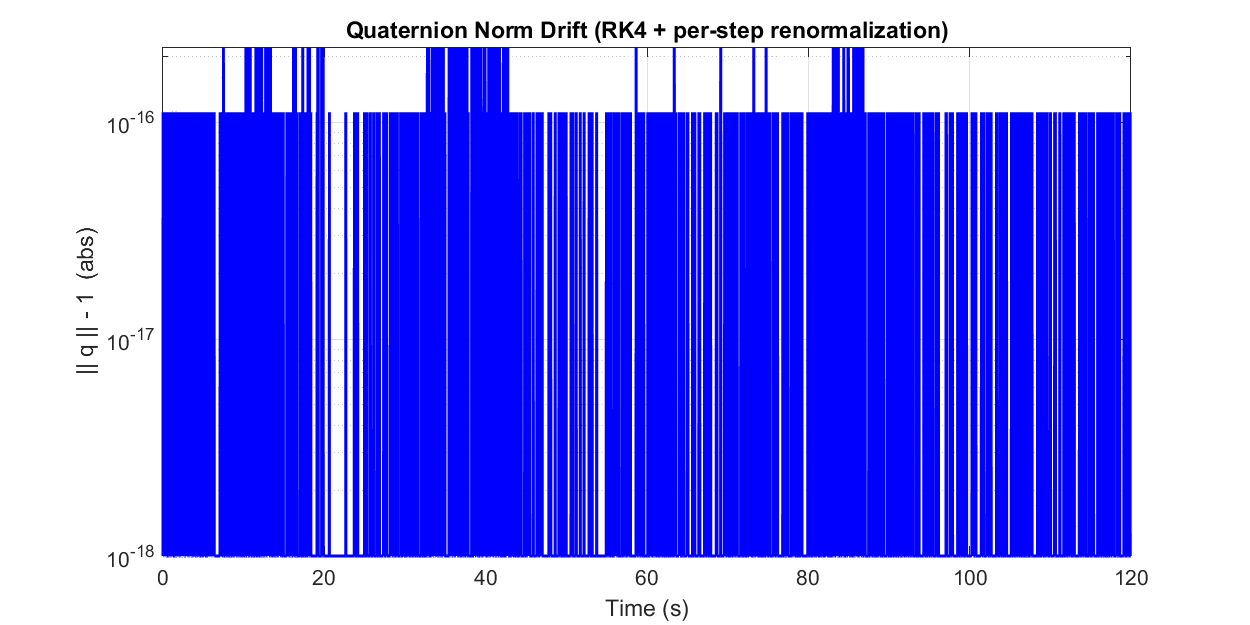
\includegraphics[width=0.72\textwidth]{fig_quaternion_norm_error.png}
\caption{Quaternion norm error.}
\label{fig:norm}
\end{figure}

\begin{figure}[htbp]
\centering
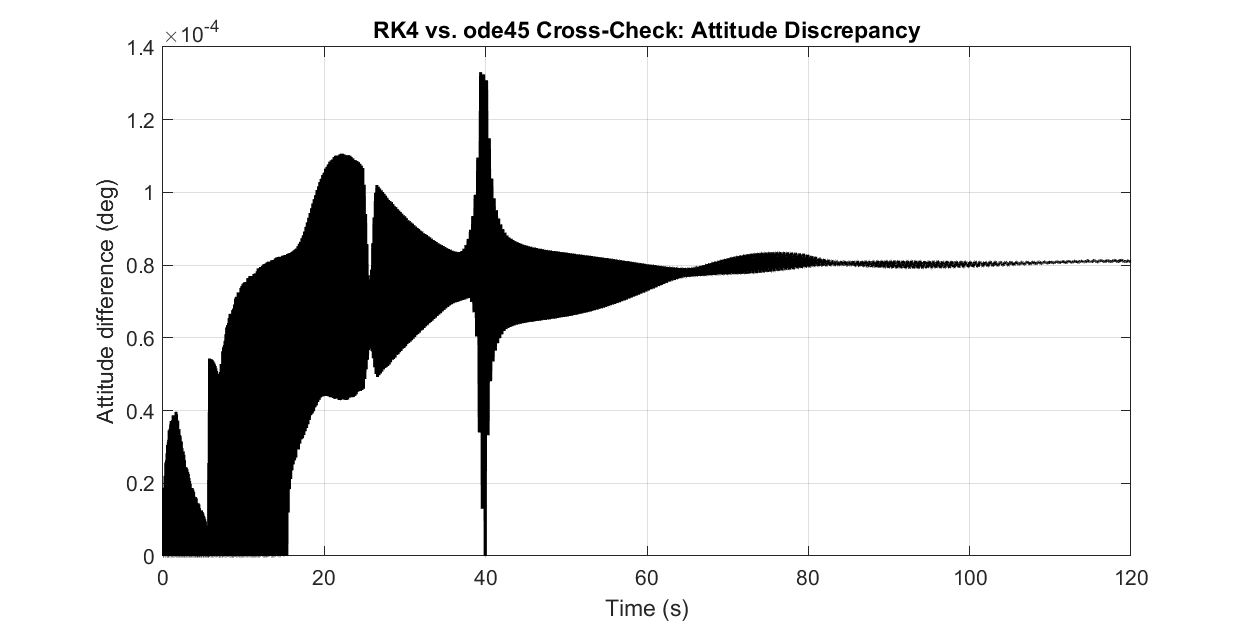
\includegraphics[width=0.72\textwidth]{fig_integrator_crosscheck.png}
\caption{Attitude difference between the RK4 and \texttt{ode45} solutions.}
\label{fig:ode45}
\end{figure}

% =====================================================================
\section{Attitude Determination with TRIAD}

In the simulation above the controller knows the exact attitude. To see how
well the attitude can be measured, I added a simple determination step. Along
the simulated trajectory, the sun direction and the magnetic field direction
are measured in the body frame with random errors of $0.1^\circ$ (sun sensor)
and $0.5^\circ$ (magnetometer), $1\sigma$. The angle between the two
reference vectors is $60^\circ$. At every step the attitude is computed with
the TRIAD method \cite{markley}, which builds two orthonormal triads from the
two vectors (the more accurate sun vector is used as the first one) and
gives the rotation matrix between them.

The results are in \figref{fig:triad}: the mean error is $0.50^\circ$, the
RMS error $0.60^\circ$ and the maximum $2.38^\circ$. A simple estimate of the
RMS error is $\sigma_{mag}/\sin(60^\circ) = 0.5^\circ/0.866 = 0.58^\circ$,
which is close to the simulated value. The error does not drift with time,
because TRIAD uses only the current measurement. In this project the
estimate is not fed back to the controller.

\begin{figure}[htbp]
\centering
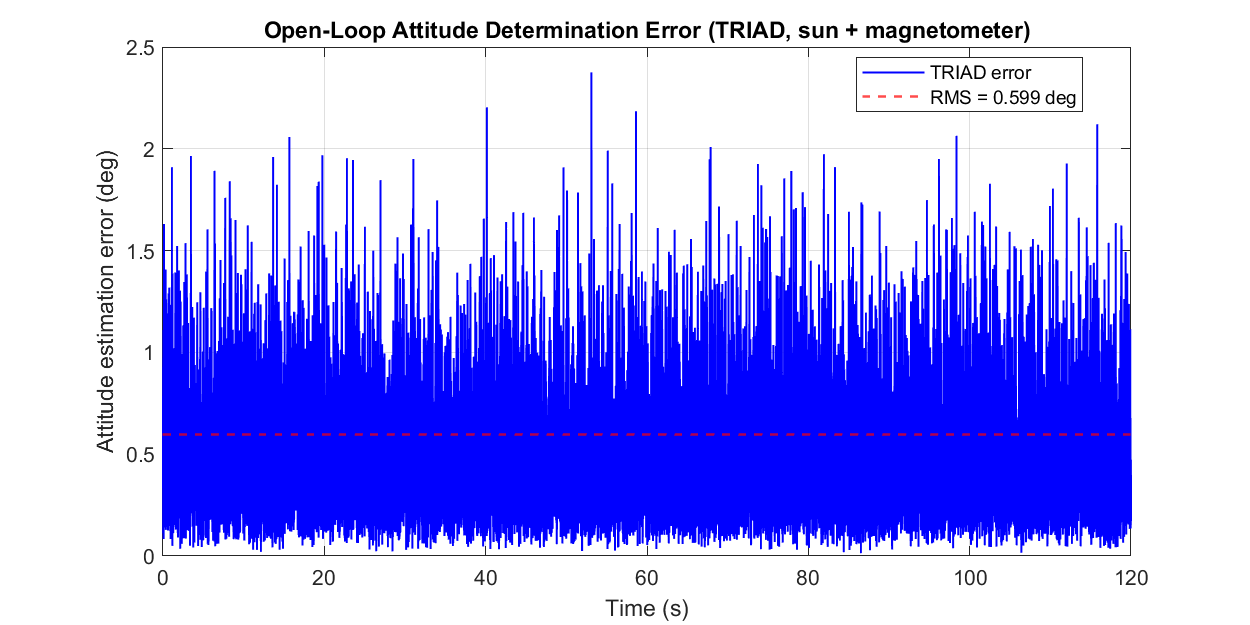
\includegraphics[width=0.72\textwidth]{fig_triad_error.png}
\caption{TRIAD attitude estimation error.}
\label{fig:triad}
\end{figure}

% =====================================================================
\section{Limitations}

\begin{itemize}[leftmargin=1.5em,itemsep=0pt]
  \item No disturbance torques. The controller was tested only for reaching a
        target, not for holding it against a constant disturbance. This is the
        most important limitation.
  \item The wheels are modeled only as a torque limit. Wheel momentum and
        momentum dumping with magnetorquers are not included.
  \item Only one initial condition and one target were simulated.
  \item The inertia comes from a uniform box model.
  \item The TRIAD estimate is not used in the control loop (no closed-loop
        estimation and control, no Kalman filter).
\end{itemize}

% =====================================================================
\section{Conclusions}

\begin{enumerate}[leftmargin=2.2em,itemsep=0pt]
  \item A quaternion PD controller with a 1~mN$\cdot$m torque limit stops a
        $19.7^\circ$/s tumble and turns a 3U CubeSat by $120^\circ$ in
        74.1~s, with a final error of $0.11^\circ$.
  \item The Lyapunov analysis shows that the PD law is stable for any
        positive gains, and the simulation confirms it: $V(t)$ decreases
        monotonically.
  \item The quaternion norm stays at one to machine precision, and RK4 and
        \texttt{ode45} agree within $1.3\times10^{-4}$ degrees.
  \item Checking the Lyapunov function in the simulation helped me find a
        wrong multiplication order in the error quaternion.
  \item Per-axis gains give the same damping on all axes, but in this case
        they make the response slightly slower (78.8~s).
  \item TRIAD with a $0.1^\circ$ sun sensor and a $0.5^\circ$ magnetometer gives
        an RMS attitude error of $0.60^\circ$.
\end{enumerate}

The next steps would be to add the gravity gradient torque, model the wheel
momentum, and use the estimated attitude in the controller with a Kalman
filter.

% =====================================================================
\begin{thebibliography}{9}
\setlength{\itemsep}{0pt}
\small

\bibitem{wertz}
Wertz, J.~R. (ed.), \textit{Spacecraft Attitude Determination and Control},
D.~Reidel, Dordrecht, 1978.

\bibitem{wie}
Wie, B., \textit{Space Vehicle Dynamics and Control}, 2nd ed., AIAA,
Reston, VA, 2008.

\bibitem{shuster}
Shuster, M.~D., ``A Survey of Attitude Representations,''
\textit{Journal of the Astronautical Sciences}, Vol.~41, No.~4, 1993,
pp.~439--517.

\bibitem{markley}
Markley, F.~L., and Crassidis, J.~L., \textit{Fundamentals of Spacecraft
Attitude Determination and Control}, Springer, New York, 2014.

\bibitem{wie_barba}
Wie, B., and Barba, P.~M., ``Quaternion Feedback for Spacecraft Large Angle
Maneuvers,'' \textit{Journal of Guidance, Control, and Dynamics}, Vol.~8,
No.~3, 1985, pp.~360--365.

\bibitem{hughes}
Hughes, P.~C., \textit{Spacecraft Attitude Dynamics}, Dover, Mineola, NY,
2004.

\bibitem{cds}
The CubeSat Program, Cal Poly SLO, \textit{CubeSat Design Specification},
Rev.~14.1, 2022.

\bibitem{bhat}
Bhat, S.~P., and Bernstein, D.~S., ``A Topological Obstruction to Continuous
Global Stabilization of Rotational Motion and the Unwinding Phenomenon,''
\textit{Systems \& Control Letters}, Vol.~39, No.~1, 2000, pp.~63--70.

\end{thebibliography}

\end{document}
